% $Id: chapter2.tex 1790 2010-09-28 16:46:40Z jabriffa $

\chapter{Literature Review}

Emotion detection problem has a problem that has been tackling alongside with the developments of Deep Learning and NLP models in recent years. 
Numerous neural network models as well as various transformers models have been suggested to solve this problem, including the papers that are going to be discussed in the following as well as it is the goal of this dissertation.

\section{What are basic emotions?}
Emotions are essential components of a human life. They are expressed in various ways which could be influence by their culture, relations, environments and so on. With all those various emotions, in emotional psychology, they are divided into two groups: basic and complex.

\begin{figure}[ht]
    \centerline{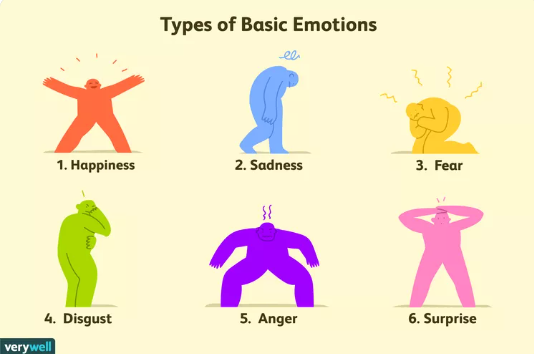
\includegraphics[scale=0.72]{Figures/six_emotions.png}}
    \caption{Six basic emotions}
    \label{fig:emotions}
 \end{figure}

For this project, we will be focussing on basic emotions. Basic emotions are emotions that are recognised them through facial expressions and tend to happen automatically \cite{Uwa_2023}. Charles Darwin is the first to proposed that the emotions that are expressed thorough facial expression are universal. Emotional psychologist, Paul Ekman identified six basic emotions: sadness, joy, fear, anger, surprise and disgust, shown in \ref{fig:emotions}. However, the purpose of this study, disgust will be replaced with love which equalises the positive and negative emotions.

\section{Why Emotion Classification?}
Research into classifying emotions across various mediums has been ongoing and evolving alongside the rapid development of new Deep Learning and NLP models. Thus, many have been polishing text emotion classification with different models such as neural networks and transformer models. However, accurately detecting emotions from text is still a goal that many are trying to reach.

The application of emotion classification, especially in medical field, could help greatly for therapist. For example, detecting a person's emotion while therapy or consultation through a chat will be a great assist for any therapist and consultant. Its application can venture into customer services as well as education (feedback for modules and lecturers)\cite{Amrullah_2023}. Other uses may include enhancement of machine translation as understanding the emotions behind the text could provide more related translation in another languages which often a struggle\cite{Amrullah_2023}. Finally, emotion based content in social media and other online platforms\cite{Amrullah_2023}. 

There are many other uses for emotion classification models and this project is to find the best suited transformer model for this task.

\section{Transformers}

\begin{figure}[ht]
    \centerline{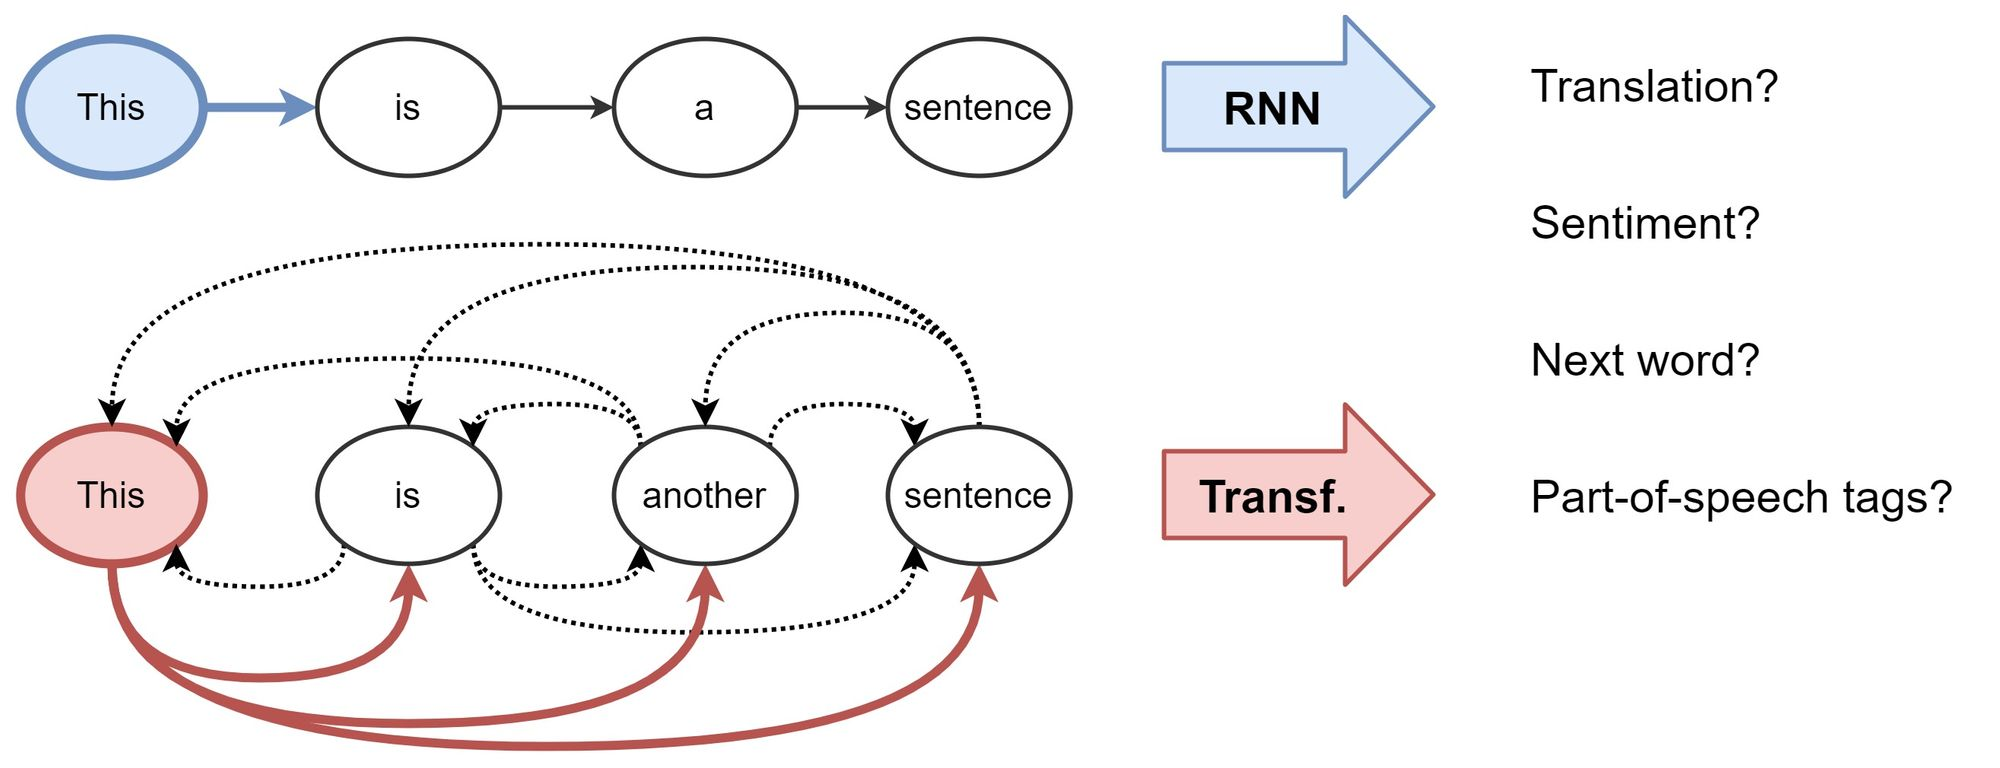
\includegraphics[scale=0.17]{Figures/rnn-transf-nlp.jpg}}
    \caption{Comparison of RNN and Transformers methods}
    \label{fig:rnn-transf}
 \end{figure}

Transformer is a model architecture that changes the world of Deep Learning and NLP to what we have now with models such as BERT based models, generative models and so on. The difference between older neural networks such as recurrent neural networks and transformer models is that rather than depending on recurrence, the model depends entirely on an attention mechanism \cite{Vaswani_Shazeer_Parmar_Uszkoreit_Jones_Gomez_Kaiser_Polosukhin_2023}. By using an attention mechanism, transformer build features of each word to figure out the importance of each word in the sentence as well as relation with each other in the given sentence like shown in Figure[\ref{fig:rnn-transf}] \cite{Vaswani_Shazeer_Parmar_Uszkoreit_Jones_Gomez_Kaiser_Polosukhin_2023}.

 \begin{figure}[ht]
    \centerline{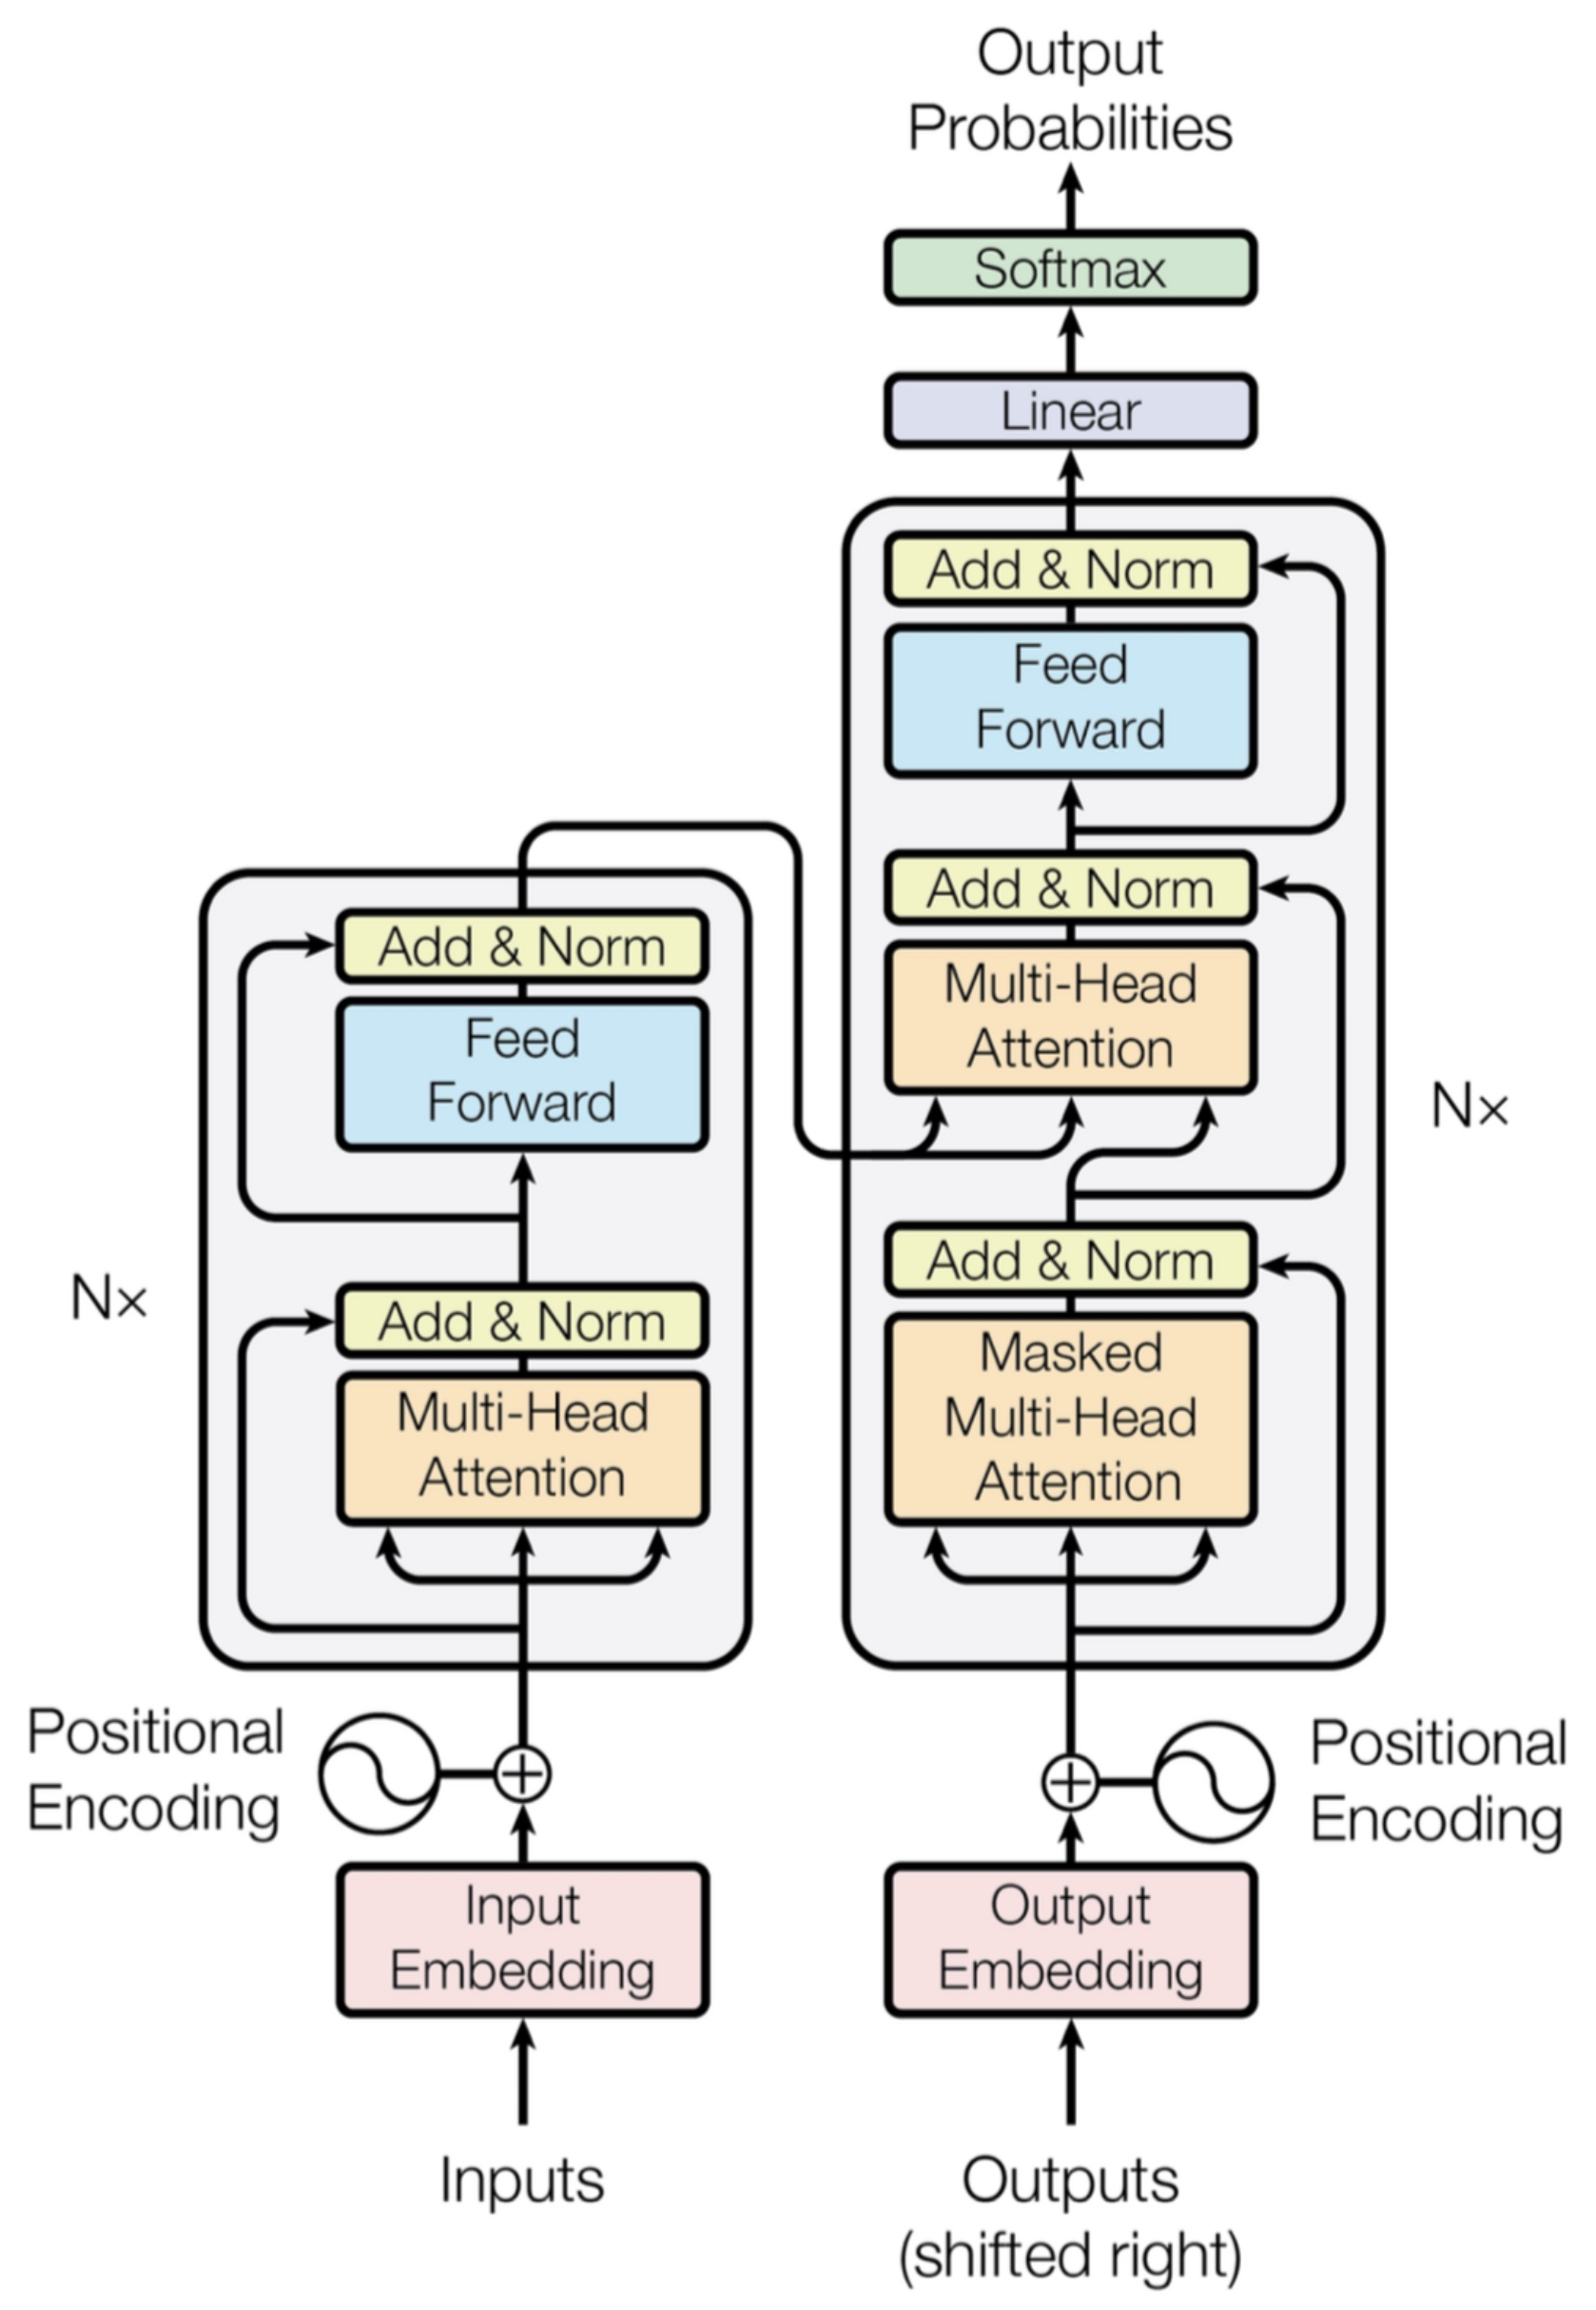
\includegraphics[scale=0.11]{Figures/encoder-decoder.jpg}}
    \caption{Architecture of Transformer}
    \label{fig:encoder-decoder}
 \end{figure}

There are many models both new and old all stem from Transformers. Such that some might only build with encoder such as BERT and BERT based models, some might only use decoder like GPT and Generative models and others might be used both encoder-decoders such as BART like the transformer architecture shown in Figure[\ref{fig:encoder-decoder}].

\subsection{BERT based models}
BERT or Bidirectional Encoder Representations from Transformers, is one of the first few variants of transformer models both in the field of deep learning and NLP.
Before BERT, language models could only read input text sequentially, which means either left-to-right or right-to-left at a time \cite{Hashemi-Pour_Lutkevich_2024}.
However, with BERT it can be done in both directions at once \cite{Hashemi-Pour_Lutkevich_2024} as a result, more contexts can be brought out and work better for text classification.

With this model, there are many variations of BERT based models, including RoBERTa and miniLM which are in the scope of this project. 

\subsubsection{RoBERTa}
RoBERTa (Robustly (optimized BERT pretraining approach)) is an improved version of BERT.
It modifies key hyperparameters, removing the next-sentence pretraining objective and training with much mini-batches and learning rates \cite{Sharma_2022}.
It is trained in much larger datasets than BERT which is under-trained. 
Furthermore, it was trained with dynamic masking, large mini-batches, larger byte-level BPE (Byte-Pair Encoding), and full-sentences without NSP (Next Sentence Prediction) loss \cite{Sharma_2022}.

Research studies have been conducted in this area, including "Multi-label emotion classification in texts using transfer learning" \cite{AMEER2023118534}. This study is using different self-attention mechanisms and then-popular, transformer models to solve the multi-label emotion classification problem.
However, because of the lack of multi-label emotion datasets, this project will be using single-label dataset.
They used two different datasets with a different set of emotion labels as well as two different languages, one of which being in English and the other in Chinese.
The transformer models they experimented with were XLNet, DistilBERT, and RoBERTa as well as multi-attention layers of each model.
Their results shown that RoBERTa with multi-attention layers (RoBERTa-MA) is the best model for multi-label emotion classification with 62.4\% accuracy and f1-score being 74.2\% and the second place with just RoBERTa which had an accuracy of 61.2\% and 73.7\% for the f1-score for English dataset. 

\subsubsection{MiniLM}

\begin{figure}[ht]
    \centerline{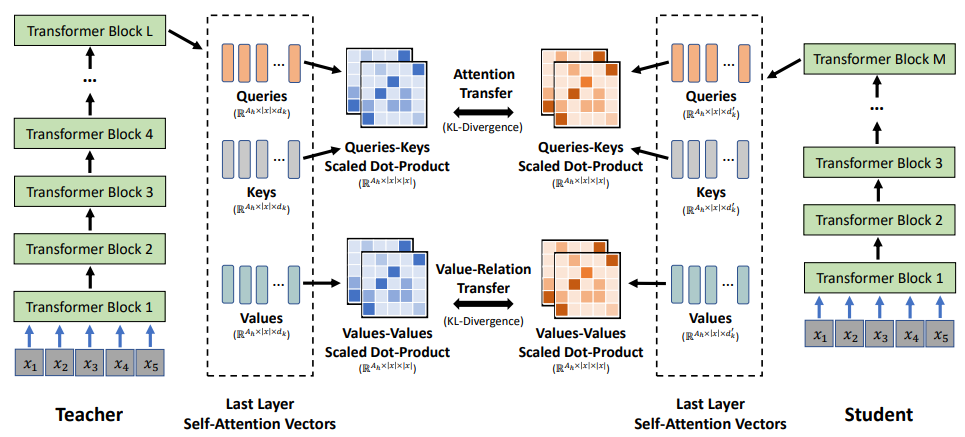
\includegraphics[scale=.5]{Figures/deep_self-distillation.png}}
    \caption{Overview of Deep Self-Attention Distillation}
    \label{fig:distillation}
 \end{figure}

Another variant of pretrained BERT is miniLM: Deep Self-attention distillation for task-agnostic compression of pretrained transformer \cite{Wang_Wei_Dong_Bao_Yang_Zhou_2020}.
It compresses large pretrained transformer based models to smaller model, otherwise called deep self-attention distillation. This means that "The small model (student) is trained by deeply mimicking the self-attention module, which play a crucial role in transformer networks, of the large model (teacher)" according to the paper \cite{Wang_Wei_Dong_Bao_Yang_Zhou_2020}, the overview shown in figure[\ref{fig:distillation}]
It also has fewer parameters than its predecessor which made it easier to fine-tune and run the model with lesser cost. 

In this paper \cite{Wang_Wei_Dong_Bao_Yang_Zhou_2020}, they may not do the same classification or the research as this project, but they fine-tuned and experimented with GLUE (General Language Understanding Evaluation) benchmark which consists of 9 sentence level classification tasks such as SQuAD2, MNLI-m, SST-2 and so-on. The average of all 8 tasks with 4 runs for each task is 80.4\% accuracy which is slightly less than BERT with 81.5\%. Nonetheless, it works better than expected for a small model.

\subsection{Llama2}
Llama stands for Large Language Model Meta AI which is a subset of LLMs which is introduced by Meta AI. Llama models vary in size, ranging from 7 billions parameters to 70 billions. The model is an autoregressive language model and based on the transformer decoder architecture. It is also a generative text model, which processes a sequence of words as input and iteratively predicts the next token using a sliding window \cite{Iraqi_2023}.

In the research article "Sentiment Analysis in the Age of Generative AI" \cite{Krugmann_Hartmann_2024}, they did 3 experiments with different classifications. The first experiment is more related to this project which is binary and three-class sentiment classification. They did the zero-shot for llama2 and GPT models using different datasets. They also compared the results with models like BERT and RoBERTa which are fine-tuned. The average accuracies of llama2, GPT-4, BERT and RoBERTa for all 16 datasets are as follows 90.9\%, 93.1\%, 90.5\% and 92.0\% respectively. The best model being GPT-4 however it is not open-source. Nevertheless, for zero-shot testing, Llama 2 did better than expected.

On the other hand, for the paper "DialogueLLM: Context and Emotion Knowledge-Tuned Large Language Models for Emotion Recognition in Conversations" \cite{zhang2024dialoguellm}, as the title suggested, it is about classifying emotion from dialogues. The datasets used have instruction, video description, context and input like Figure[\ref{fig:DialogueLLM}] and the output will be single emotion. They used other models such as MTL, Llama2 to compare with their model DialogueLLM. The results for Llama2 are significantly lower than the article above, with average accuracy being 25.31\% and f1-score being 21.91\%. In which their best model being DialogueLLM with 61.4\% and 60.52\% respectively. This suggested that Llama2 is not suitable for extracting emotion from the dialogue based input. 
\begin{figure}[!htb]
    \centerline{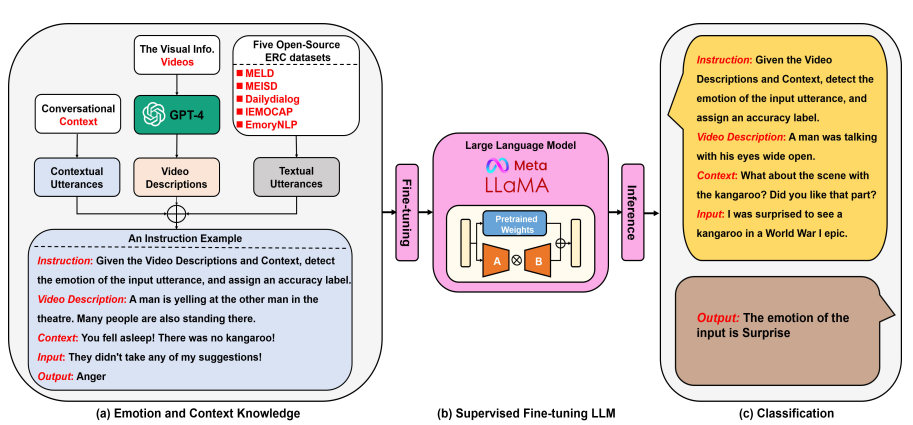
\includegraphics[scale=.68]{Figures/dialogueLLM.png}}
    \caption{Overview of DialogueLLM fine-tuning and classification pipeline from the paper mentioned above}
    \label{fig:DialogueLLM}
 \end{figure}

\subsection{GPT}
 GPT (Generative pretrained transformer) is a series of language models that is developed by OpenAI \cite{Jorge_2023}. GPT have 4 different versions: GPT, GPT-2, GPT-3.5 and GPT4. The latest two versions may not open-sourced however the public could still use GPT-1 and 2 to experiment or compare with the newly developments of LLMs. GPT shines mainly in text generation which produces coherent and contextually relevant sentences \cite{Jorge_2023}.
 
 For the related research for this model, "Generative Pretrained Transformers for Emotion Detection in a Code-Switching Setting" \cite{Nedilko}, they used GPT models with the zero-shot or few-shot approaches to detect the human emotions. As they could not access GPT-4, they used ChatGPT for this experiment with few-shot-method and got 73.13\% for the accuracy and 70.38\% for the macro-f1. If there is access for GPT-4 as shown in the previous paper above, the result of this experiment will be greater.
 
 \section{Overall}

 Most of the models, especially RoBERTa, Llama2 and GPT-2 shown that they might be suitable for downstream task such as emotion classification. Their accuracy and f1-score are mostly above 60\%. Therefore, this project's purpose is to experiment with these models, fine-tuned them according to my dataset and, evaluate and test the model to find out which model is the best suited for the emotion detection task.

 For miniLM, it may not have any paper regarding with emotion classification, the project's aim is to also find possible model for emotion classification. In which miniLM's methods and size and results of GLUE benchmark, it is included in this project's experimentation.
 
The following chapters will dive into the implementation of each model, the dataset, and how the results from the implementation will be compared and analysed as well as their methodologies and limitations will be explained.